\documentclass[conference]{IEEEtran}
\IEEEoverridecommandlockouts
\usepackage{graphicx}
\usepackage{booktabs}
\usepackage{url}
\usepackage{hyperref}
\usepackage{amsmath}
\usepackage{amssymb}
\usepackage{float}
\usepackage{caption}

\title{Tech Workforce Cycles in the Era of Generative AI:
A Data-Driven Analysis of Layoffs, Hiring Dynamics, and Occupational Reallocation (2017–2026)}

\author{
\IEEEauthorblockN{Seu Nome}
\IEEEauthorblockA{
Sua Instituição \\
Email: seu@email.com
}
}

\begin{document}
\maketitle

% ==============================
\begin{abstract}

Public discourse frequently associates the rise of Generative AI with mass layoffs in the technology sector. This study evaluates that hypothesis using official labor-flow data from the U.S. Bureau of Labor Statistics (BLS) Job Openings and Labor Turnover Survey (JOLTS), focusing on the Information sector (NAICS 51) as a measurable proxy for technology-adjacent industries. We analyze monthly hires and layoffs between 2017 and 2026, identify structural peaks and valleys, and annotate them with macroeconomic shocks, financial tightening cycles, and major AI milestones. Our findings suggest that workforce contraction aligns more strongly with capital-cycle corrections and post-pandemic over-hiring adjustments than with AI releases themselves. However, occupational composition shifts toward AI, data, and cybersecurity roles indicate structural reallocation rather than net labor collapse.

\end{abstract}

\begin{IEEEkeywords}
JOLTS, NAICS 51, layoffs, hiring rate, generative AI, labor reallocation, workforce cycles
\end{IEEEkeywords}

% ==============================
\section{Introduction}

Since the public launch of ChatGPT in November 2022, narratives have emerged linking Generative AI tools to widespread job displacement in the technology sector. While large-scale layoffs occurred in 2023–2024, attributing them directly to AI risks conflating technological adoption with macroeconomic contraction.

This paper evaluates labor-flow evidence using official U.S. data to determine whether:
\begin{itemize}
\item Layoff waves temporally align with AI milestones;
\item Hiring collapses structurally after Generative AI release;
\item Workforce shifts reflect technological substitution or macroeconomic correction.
\end{itemize}

% ==============================
\section{Data and Sector Definition}

\subsection{JOLTS Overview}

The Job Openings and Labor Turnover Survey (JOLTS) measures:
\begin{itemize}
\item Hires
\item Layoffs and discharges
\item Job openings
\end{itemize}

We use monthly non-seasonally adjusted data.

\subsection{Why NAICS 51?}

NAICS 51 (Information) includes:
\begin{itemize}
\item Software publishing
\item Telecommunications
\item Data processing services
\item Media and digital infrastructure
\end{itemize}

While not equivalent to “Big Tech,” it represents the closest consistently measurable proxy for tech-adjacent industries.

% ==============================
\section{Methodology}

\subsection{Peak and Valley Detection}

Given a time series $x_t$, a point $t$ is classified as:

Peak:
\[
x_t = \max(x_{t-k}, ..., x_{t+k})
\]

Valley:
\[
x_t = \min(x_{t-k}, ..., x_{t+k})
\]

with window size $k=3$ months.

\subsection{Projection Model}

We compute a linear regression on the last six observations:

\[
\hat{y}_t = \beta_0 + \beta_1 t
\]

Confidence interval (naive approximation):

\[
\hat{y}_t \pm 1.96\sigma
\]

where $\sigma$ is residual standard deviation.

% ==============================
\section{Empirical Results}

\subsection{Layoffs (Level, Thousands)}

\begin{figure}[H]
\centering
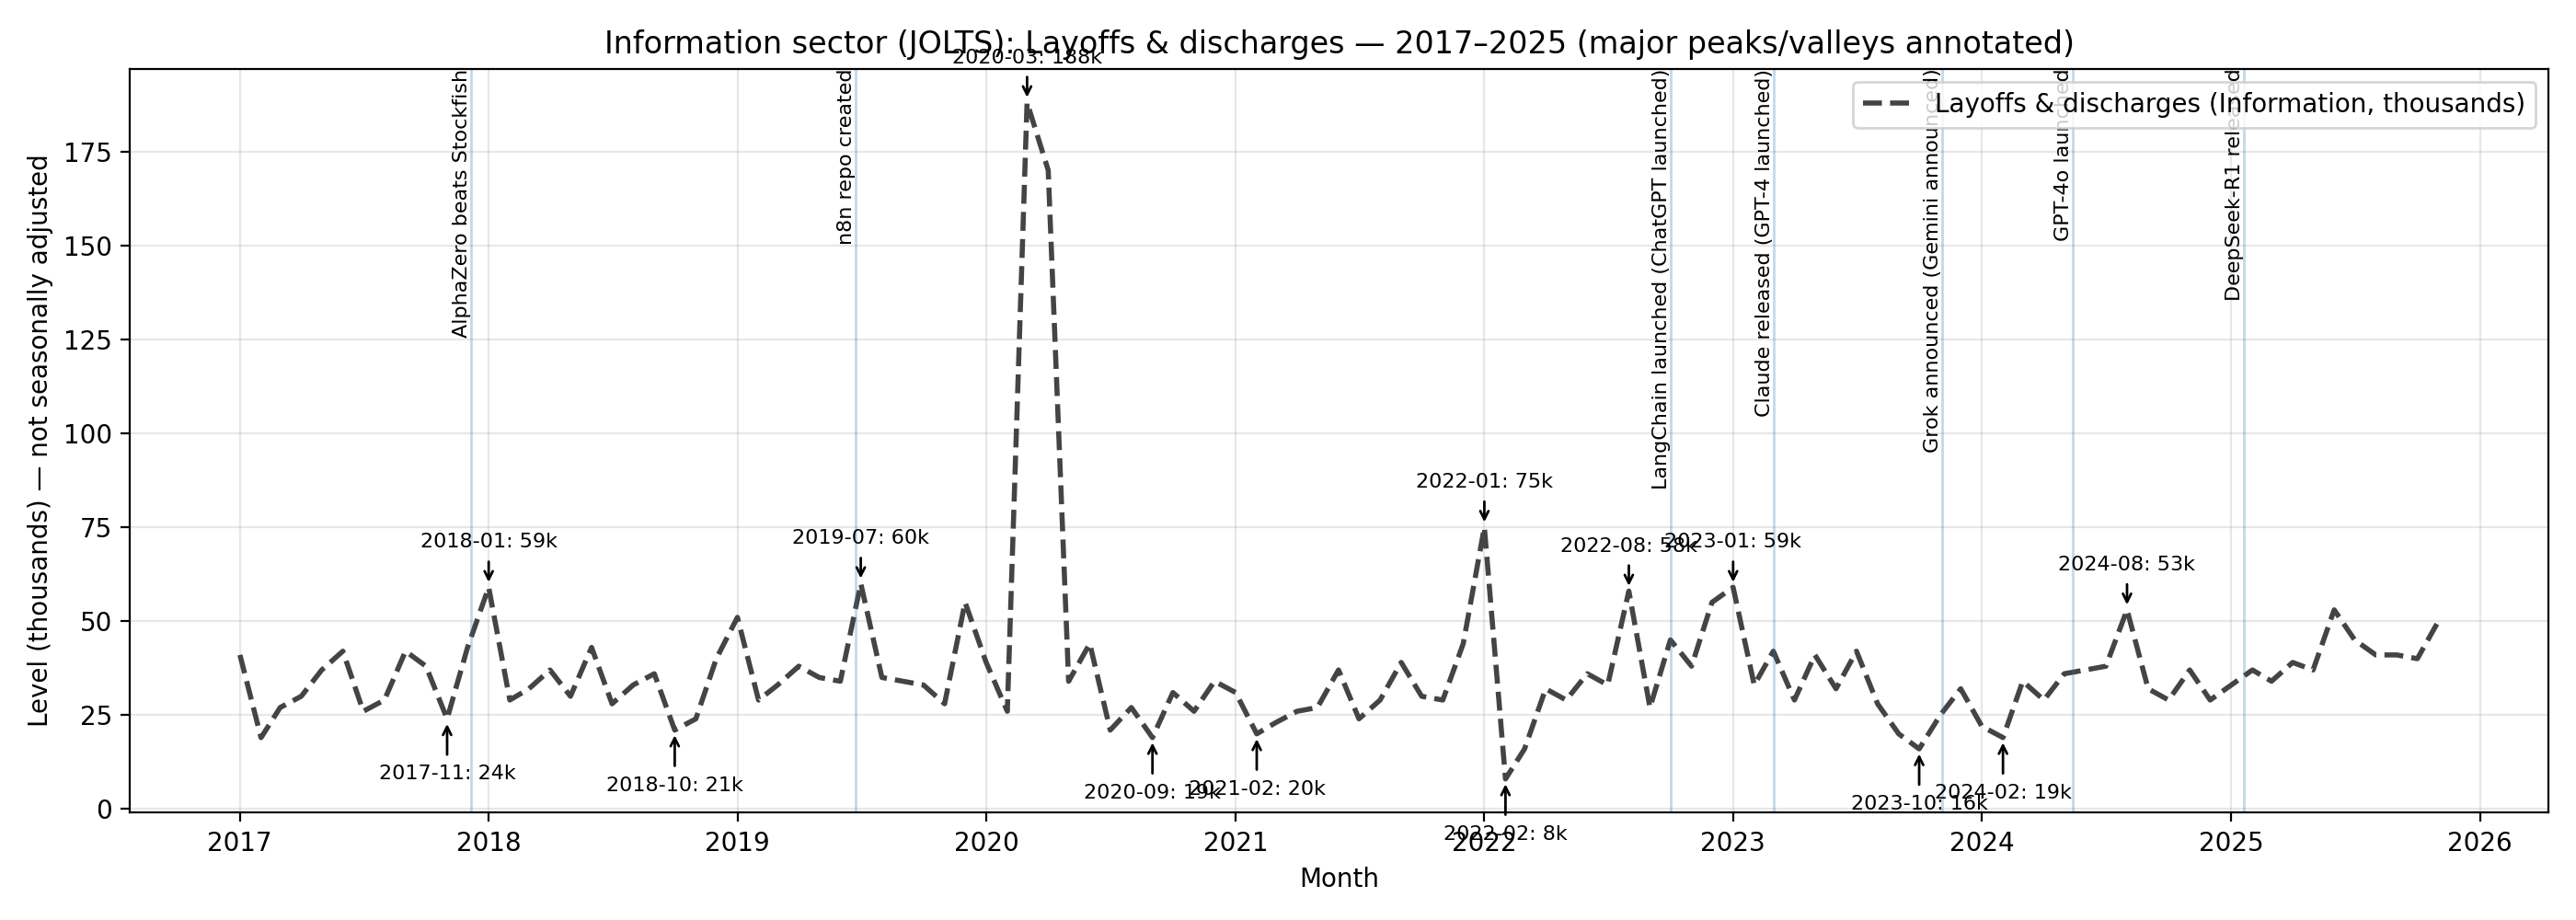
\includegraphics[width=\linewidth]{jolts_information_layoffs_only_2017_2025.png}
\caption{Layoffs and discharges (Information sector).}
\end{figure}

Major peaks align with:
\begin{itemize}
\item COVID lockdown shock (2020)
\item Federal Reserve tightening cycle (2022–2023)
\item Venture capital contraction and SVB collapse (2023)
\end{itemize}

No major structural spike aligns directly with GPT-4 or Gemini releases.

\subsection{Hiring Rate (\%)}

\begin{figure}[H]
\centering
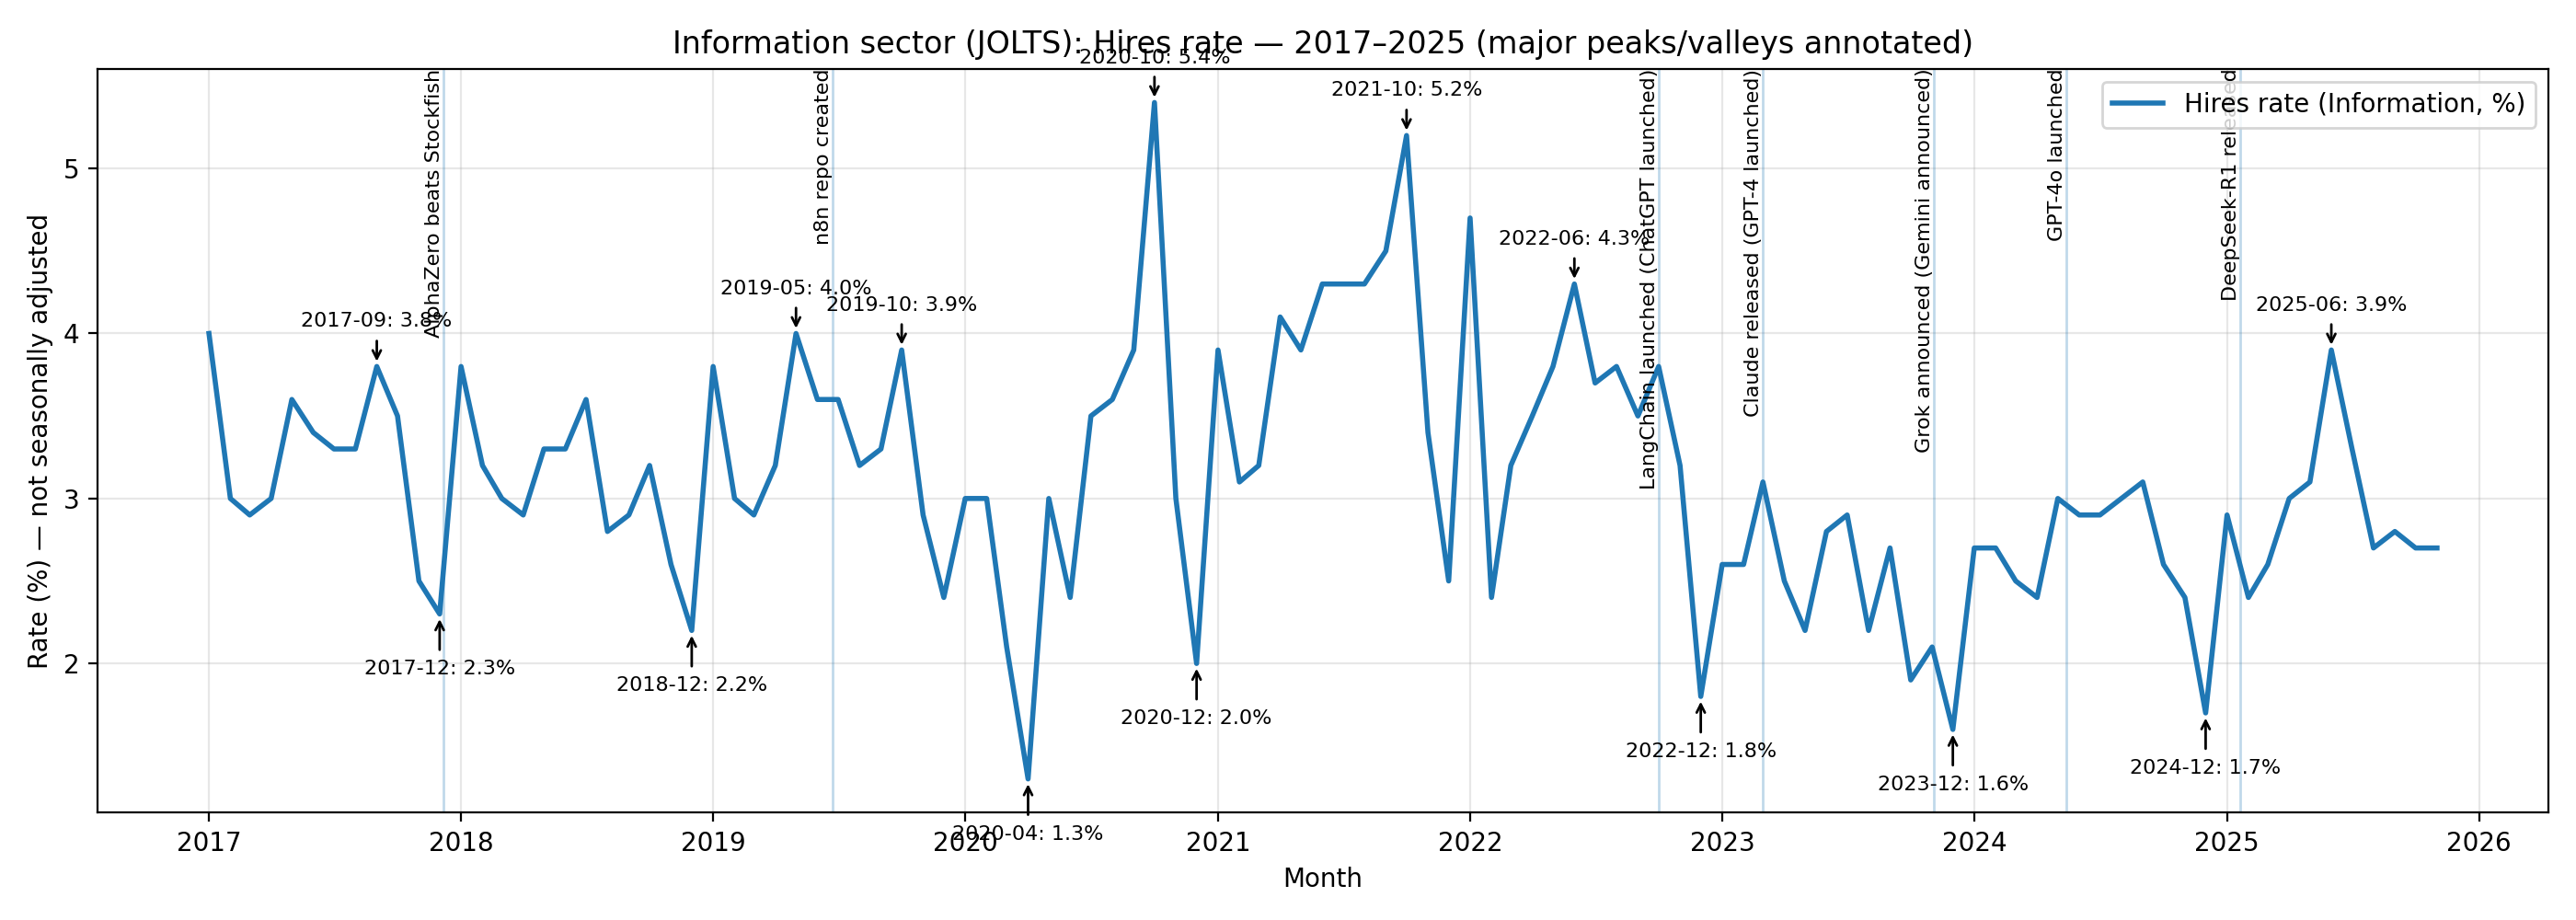
\includegraphics[width=\linewidth]{jolts_information_hires_rate_only_2017_2025.png}
\caption{Hires rate (Information sector).}
\end{figure}

Hiring declines gradually during tightening cycles but does not collapse after AI milestones.

% ==============================
\section{Macro vs AI Attribution}

Key macro factors:
\begin{itemize}
\item Rising interest rates (capital cost shock)
\item Post-pandemic over-hiring correction
\item Venture capital pullback
\end{itemize}

Generative AI appears to:
\begin{itemize}
\item Shift role composition
\item Increase demand for AI/ML specialists
\item Reduce repetitive clerical demand
\end{itemize}

% ==============================
\section{Occupational Reallocation}

Reports from WEF and LinkedIn show growth in:

\begin{itemize}
\item AI/ML Specialists
\item Data Scientists
\item Cybersecurity Specialists
\item Software Developers
\end{itemize}

Declining roles:
\begin{itemize}
\item Clerical positions
\item Data entry
\item Repetitive administrative functions
\end{itemize}

This suggests reallocation rather than structural collapse.

% ==============================
\section{Projection Analysis}

\begin{figure}[H]
\centering
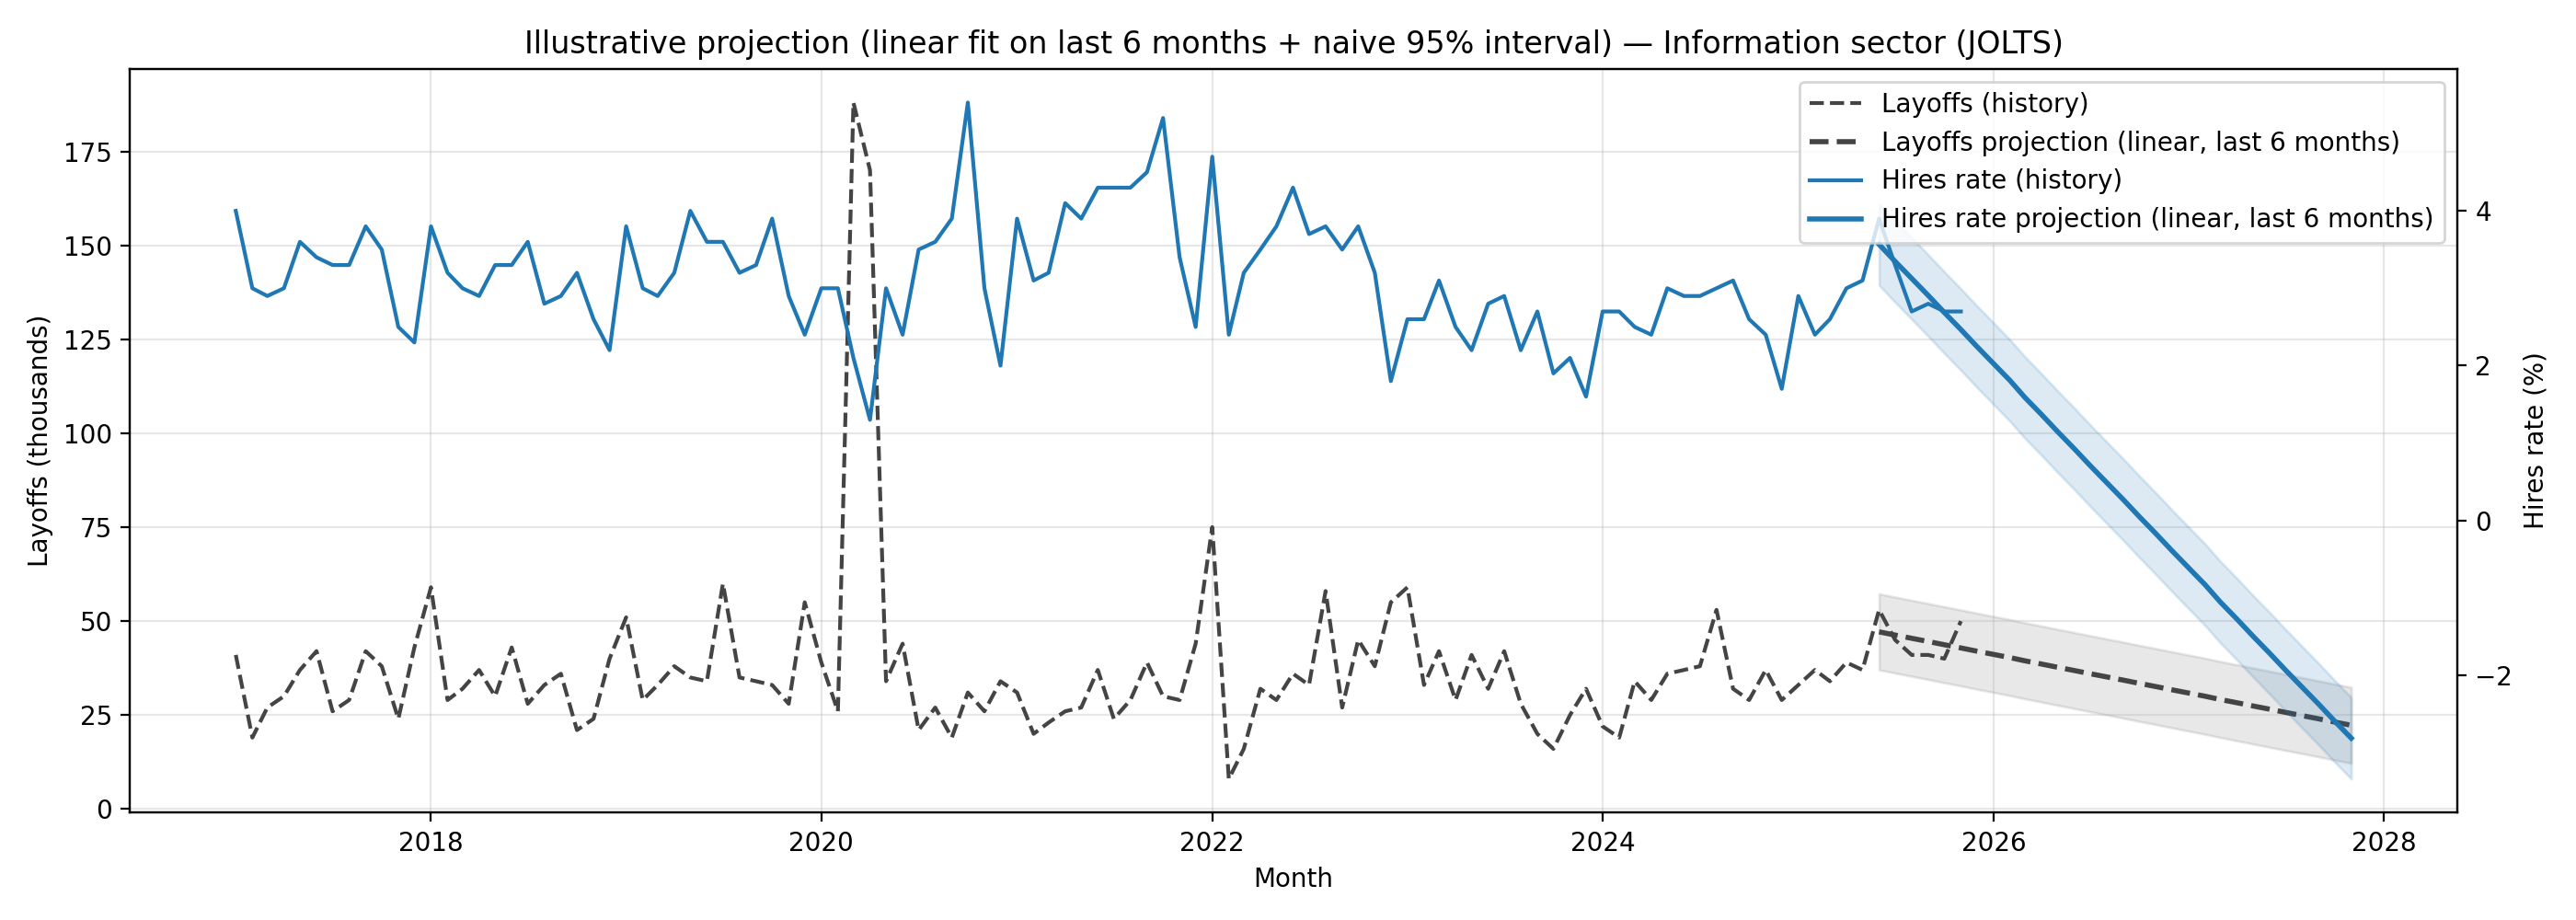
\includegraphics[width=\linewidth]{jolts_information_projection_last6mo_with_ci.png}
\caption{Illustrative projection (linear trend).}
\end{figure}

Projection suggests stabilization rather than acceleration of layoffs.

% ==============================
\section{Limitations}

\begin{itemize}
\item NAICS 51 is proxy, not pure Big Tech
\item Hires used as rate, not absolute level
\item Projection model is illustrative, not structural
\item Causality cannot be inferred from correlation
\end{itemize}

% ==============================
\section{Conclusion}

Evidence indicates that:
\begin{itemize}
\item Layoff waves align primarily with macroeconomic tightening.
\item AI milestones do not directly trigger structural spikes.
\item Workforce reallocation toward AI-centric roles is observable.
\item Generative AI reshapes demand composition rather than eliminating tech employment.
\end{itemize}

The labor market transition is cyclical and structural, not purely technological.

\bibliographystyle{IEEEtran}
\bibliography{references}

\end{document}